\documentclass{article}
\usepackage[utf8]{inputenc}
\usepackage{longtable}
\usepackage{tikz}
\usetikzlibrary{arrows.meta}

% From https://tex.stackexchange.com/q/89129
\makeatletter
\newcount\dirtree@lvl
\newcount\dirtree@plvl
\newcount\dirtree@clvl
\def\dirtree@growth{%
    \ifnum\tikznumberofcurrentchild=1\relax
      \global\advance\dirtree@plvl by 1
      \expandafter\xdef\csname dirtree@p@\the\dirtree@plvl\endcsname{\the\dirtree@lvl}
    \fi
    \global\advance\dirtree@lvl by 1\relax
    \dirtree@clvl=\dirtree@lvl
    \advance\dirtree@clvl by -\csname dirtree@p@\the\dirtree@plvl\endcsname
    \pgf@xa=1cm\relax
    \pgf@ya=-0.6cm\relax
    \pgf@ya=\dirtree@clvl\pgf@ya
    \pgftransformshift{\pgfqpoint{\the\pgf@xa}{\the\pgf@ya}}%
    \ifnum\tikznumberofcurrentchild=\tikznumberofchildren
        \global\advance\dirtree@plvl by -1
    \fi
}

\tikzset{
  dirtree/.style={
    growth function=\dirtree@growth,
    growth parent anchor=south west,
    parent anchor=south west,
    every child node/.style={anchor=west},
    edge from parent path={([xshift=2ex] \tikzparentnode\tikzparentanchor) 
                           |- (\tikzchildnode\tikzchildanchor)}
  }
}

\title{EigenpackConvert Documentation}
\author{Ryan Hill\\ Ryan.Hill@ed.ac.uk}
\begin{document}
\maketitle
\tableofcontents
\newpage
\section{File Format Specification}
\subsection{Overview}
The GPT Eigenpack multifile format describes lattice eigenvectors generated under the ``Local Coherence" scheme. Under this scheme, the lattice (or as we will describe it going forwards, the \textbf{fine grid}) is coarsened into a \textbf{coarse grid}, as exemplified for 2D in Figure~\ref{FIGURE::LocalCoherenceCoarsening} with a coarsening of 3 in both the x and y dimensions. In Figure~\ref{FIGURE::LocalCoherenceCoarsening}, sites 0, 1, 2, 9, 10, 11, 18, 19, and 20 are associated with the coarse site 0, with other associations illustrated by the figure also. Data is similarly associated (but much harder to draw) for the 4D or 5D lattice data we are interested in. For each \textbf{fine site}, a limited number of eigenvectors are stored. We will refer to these as \textbf{basis vectors}. Typically, a substantially larger number of eigenvectors are then expressed as a \textbf{set of coefficients} of these \textbf{basis vectors} on each \textbf{coarse site}. The larger set of eigenvectors can then be generated per \textbf{fine site} by taking the dot product of the \textbf{fine site}'s set of \textbf{basis vectors} with the \textbf{coarse coefficients} for that \textbf{fine site}'s corresponding \textbf{coarse site}. Since the eigenvectors of similarly-situated lattice sites are highly correlated (or ``\textbf{locally coherent}"), this is a good approximation of the true set of eigenvectors per \textbf{fine site}. We therefore have two pieces of data to keep track of: \textbf{basis vectors} for each \textbf{fine site}, and \textbf{coarse coefficients} for each \textbf{coarse site}.\\

\begin{figure}
\label{FIGURE::LocalCoherenceCoarsening}
\begin{center}
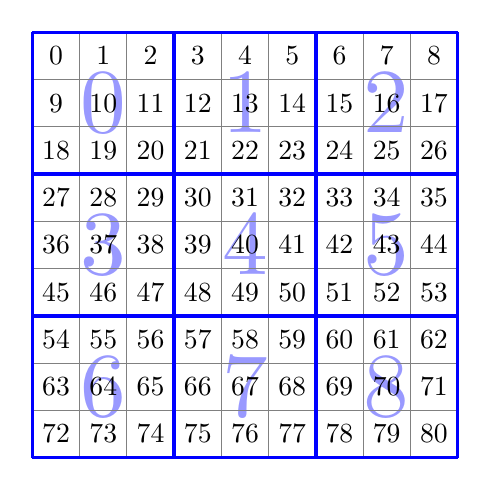
\begin{tikzpicture}[scale=0.6]
\clip (-0.1,-0.1) rectangle (9.1,9.1);

% Big blue numbers
\foreach \y [count=\ny from 0] in {7.5, 4.5, 1.5} {
  \foreach \x [count=\nx from 0, evaluate=\x as \num using int(\nx + (\ny)*3)] in {1.5, 4.5, 7.5} {
    \node[text=blue, scale=3.3, opacity=0.4, inner sep=0.1cm,outer sep=0pt,anchor=center, minimum size=1cm] at (\x,\y) {\num};
  }
}

% Grids
\draw [step=1.0,gray, thin] (0,0) grid (9,9);
\draw [step=3.0,blue, very thick] (0,0) grid (9,9);

% Small black numbers
\foreach \y [count=\ny from 0] in {8.5,7.5,...,0.5} {
  \foreach \x [count=\nx from 0, evaluate=\x as \num using int(\nx + (\ny)*9)] in {0.5,1.5,...,8.5} {
    \node[inner sep=0.1cm,outer sep=0pt,anchor=center, minimum size=1cm] at (\x,\y) {\num};

  }
}
\end{tikzpicture}
\end{center}
\caption{Allocation of fine sites to coarse sites in the GPT Eigenpack.}
\end{figure}
\noindent
The \textbf{block} is the organisational unit of the GPT Eigenpack format. A \textbf{block} comprises the set of \textbf{coarse coefficients} for a particlar \textbf{coarse site} in addition to the \textbf{basis vectors} for each \textbf{fine site} covered by the \textbf{coarse site}. These \textbf{blocks} are then grouped into \textbf{volumes}, where (similarly to how \textbf{fine sites} are grouped into \textbf{blocks}) each \textbf{volume} covers a consistent number of \textbf{blocks} in each dimension. Each \textbf{volume} is stored as a separate \textbf{file}. This makes the GPT Eigenpack highly efficient to load when the local volume of the compute nodes exactly factorises into the volumes covered by each Eigenpack \textbf{file}, since since this permits perfect parallelism where two nodes will never need to access the same \textbf{file} during I/O. These \textbf{files} are also equally distributed between 32 \textbf{directories}.

\subsection{Float Compression}
In addition to the compression obtained by using the Local Coherence scheme for storing eigenvectors, a further step of compression is supported by allowing the least significant basis vectors to be stored with reduced precision. This ``reduced precision" format is defined in terms of 

\subsection{Specification Details}

\subsubsection{Metadata}
The Metadata file is an ASCII plaintext file with key-value pairs given in format
\begin{center}
\textless key\textgreater\space=\space\textless value\textgreater 
\end{center}
Tabulated below are a list of identifiers and a variable name used in subsequent sections to refer to the value of this identifier. All values are unsigned integers.

\begin{longtable}{p{.2\textwidth} |p{.21\textwidth} |p{.59\textwidth}}
\hline
Name & Variable Name & Description\\
\hline
s[0] &  & The total number of fine sites in the X dimension contained in each eigenvector file.\\
s[1] &  & The total number of fine sites in the Y dimension contained in each eigenvector file.\\
s[2] &  & The total number of fine sites in the Z dimension contained in each eigenvector file.\\
s[3] &  & The total number of fine sites in the T dimension contained in each eigenvector file.\\
s[4] &  & The total number of fine sites in the Ls dimension contained in each eigenvector file.\\
b[0] & \hfil x & The total number of fine sites in the X dimension contained in each block.\\
b[1] & \hfil y & The total number of fine sites in the Y dimension contained in each block.\\
b[2] & \hfil z & The total number of fine sites in the Z dimension contained in each block.\\
b[3] & \hfil t & The total number of fine sites in the T dimension contained in each block.\\
b[4] & \hfil Ls & The total number of fine sites in the Ls dimension contained in each block.\\
nb[0] & \hfil xBlock & The total number of blocks in the X dimension contained in each eigenvector file. This is equal to s[0]/b[0].\\
nb[1] & \hfil yBlock & The total number of blocks in the Y dimension contained in each eigenvector file. This is equal to s[1]/b[1].\\
nb[2] & \hfil zBlock & The total number of blocks in the Z dimension contained in each eigenvector file. This is equal to s[2]/b[2].\\
nb[3] & \hfil tBlock & The total number of blocks in the T dimension contained in each eigenvector file. This is equal to s[3]/b[3].\\
nb[4] & \hfil LsBlock & The total number of blocks in the Ls dimension contained in each eigenvector file. This is equal to s[4]/b[4].\\
neig & eigenvectorCount & The total number of eigenvectors stored as coefficients of coarse grid sites.\\
nkeep\_single & \hfil fp32BasisCount & The number of basis vectors on each fine site stored in single precision.\\
nkeep & & The total number of basis vectors on each fine site. The number of compressed basis vectors on each fine site (referred to as fp16BasisCount below) is defined by $n_\mathrm{keep} - n_\mathrm{keep}^\mathrm{single}$\\
blocks & & The total number of blocks stored per file. This is equal to nb[0]*nb[1]*nb[2]*nb[3]*nb[4].\\
FP16\_COEF\_ EXP\_SHARE\_ FLOATS & & The number of eigenvector coefficients for the compressed basis vectors that are compressed using the same scaling factor.\\
crc32[$i$] & & The crc32 checksum for data file $i$.\\
\hline
\end{longtable}

\subsubsection{Compressed File}
\begin{tabular}{p{.2\textwidth} |p{.4\textwidth} |p{.4\textwidth}}
\hline
Name & Type & Description\\
\hline
basisFP32 & BasisVectors[LsBlock][tBlock] [zBlock][yBlock][xBlock] [fp32BasisCount] & A list of basis vectors stored in single precision for each block contained within the file.\\
basisFP16 & CompressedBasisVectors [LsBlock][tBlock][zBlock] [yBlock][xBlock] [fp16BasisCount] & A list of additional basis vectors stored in a compressed format for each block contained within the file.\\
coefficients & Coefficients[eigenvectorCount]
[LsBlock][tBlock][zBlock] [yBlock][xBlock]  & A list of coefficients used to reconstruct eigenvectors by taking their product with the basis vectors. One set of coefficients is stored per eigenvector per block.\\
\hline
\end{tabular}

\subsubsection{BasisVectors}
\begin{tabular}{p{.2\textwidth} |p{.4\textwidth} |p{.4\textwidth}}
\hline
Name & Type & Description\\
\hline
sites & LatticeFermion[Ls][t][z][y][x] & One Basis Vector on each fine lattice site in the given block. The five dimensions given in the type are the extent of the fine grid that a block covers.\\
\hline
\end{tabular}

\subsubsection{LatticeFermion}
\begin{tabular}{p{.2\textwidth} |p{.4\textwidth} |p{.4\textwidth}}
\hline
Name & Type & Description\\
\hline
elements & float[4][3][2] & Elements of a SpinColourMatrix. The three dimensions are Spin, Colour, and complex components.\\
\hline
\end{tabular}

\subsubsection{CompressedBasisVectors}
\begin{tabular}{p{.2\textwidth} |p{.4\textwidth} |p{.4\textwidth}}
\hline
Name & Type & Description\\
\hline
sites & CompressedLatticeFermion [Ls][t][z][y][x] & Compressed data for one Basis Vector on each fine lattice site in the given block. The five dimensions given in the type are the extent of the fine grid that a block covers.\\
\hline
\end{tabular}

\subsubsection{CompressedLatticeFermion}
\begin{tabular}{p{.2\textwidth} |p{.4\textwidth} |p{.4\textwidth}}
\hline
Name & Type & Description\\
\hline
elements & CompressedFloats\textless 24\textgreater & Elements of a SpinColourMatrix. The elements are arranged in the same order as the LatticeFermion elements. \\
\hline
\end{tabular}

\subsubsection{CompressedFloats\textless size\textgreater}
\begin{tabular}{p{.2\textwidth} |p{.4\textwidth} |p{.4\textwidth}}
\hline
Name & Type & Description\\
\hline
exponent & uint16 & The common scale for all elements.\\
elements & int16[size] &  Two bytes per compressed float held by the struct. Refer to \ref{} to see how to compress and de-compress the elements of this format to floats.\\
\hline
\end{tabular}

\subsubsection{Coefficients}
\begin{tabular}{p{.2\textwidth} |p{.4\textwidth} |p{.4\textwidth}}
\hline
Name & Type & Description\\
\hline
fp32Coefs & float[fp32BasisCount][2] & Coefficients for the uncompressed basis vectors. Each coefficient is complex and is represented by two floats.\\
fp16Coefs & CompressedFloats\textless 10\textgreater\space [2$*$fp16BasisCount/10] & Coefficients for the compressed basis vectors. The coefficients are stored in chunks of 10, with each chunk stored in a CompressedFloats\textless 10\textgreater\space struct. Each coefficient is complex and is represented by two floats.\\
\hline
\end{tabular}

\iffalse
\begin{figure}
\begin{center}
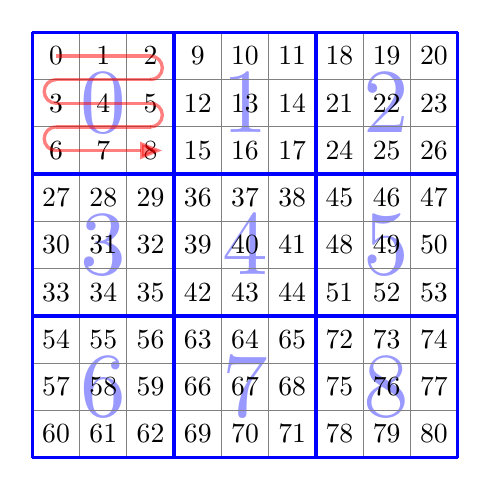
\begin{tikzpicture}[scale=0.6]
\clip (-0.1,-0.1) rectangle (9.1,9.1);

% Big blue numbers
\foreach \y [count=\ny from 0] in {7.5, 4.5, 1.5} {
  \foreach \x [count=\nx from 0, evaluate=\x as \num using int(\nx + (\ny)*3)] in {1.5, 4.5, 7.5} {
    \node[text=blue, scale=3.3, opacity=0.4, inner sep=0.1cm,outer sep=0pt,anchor=center, minimum size=1cm] at (\x,\y) {\num};
  }
}

% Grids
\draw [step=1.0,gray, thin] (0,0) grid (9,9);
\draw [step=3.0,blue, very thick] (0,0) grid (9,9);

% Small black numbers
\foreach \yblock [count=\nyblock from 0] in {6,3,0} {
  \foreach \xblock [count=\nxblock from 0, evaluate=\xblock as \numblock using int(\nxblock + (\nyblock)*3)] in {0,3,6} {
      \foreach \y [count=\ny from 0] in {2.5,1.5,0.5} {
        \foreach \x [count=\nx from 0, evaluate=\x as \num using int(\nx + (\ny)*3 + 9*\numblock)] in {0.5,1.5,2.5} {
        \node[inner sep=0.1cm,outer sep=0pt,anchor=center, minimum size=1cm] at (\xblock+\x,\yblock+\y) {\num};
      }
    }
  }
}

% Arrow
\draw [color=red, very thick, opacity=0.5] (0.5,8.5) -- (2.5,8.5);
\draw [color=red, very thick, opacity=0.5] (2.5,8.0) arc (-90:90:0.25);
\draw [color=red, very thick, opacity=0.5] (2.5,8.0) -- (0.5, 8.0);
\draw [color=red, very thick, opacity=0.5] (0.5,8.0) arc (-90:90:-0.25);
\draw [color=red, very thick, opacity=0.5] (0.5,7.5) -- (2.5,7.5);
\draw [color=red, very thick, opacity=0.5] (2.5,7.0) arc (-90:90:0.25);
\draw [color=red, very thick, opacity=0.5] (2.5,7.0) -- (0.5, 7.0);
\draw [color=red, very thick, opacity=0.5] (0.5,7.0) arc (-90:90:-0.25);
\draw [-{Triangle[length=8pt,width=6pt]}, color=red, very thick, opacity=0.5] (0.5,6.5) -- (2.75,6.5);
\end{tikzpicture}
\end{center}
\end{figure}
\fi

\clearpage
\section{Program Specification}
\subsection{Overview}
This program is designed to convert a GPT Eigenpack into a Scidac Eigenpack, using Grid and Hadrons to define the Scidac Eigenpack data structure and to write it to disk.\\
\textbf{Note: The program will only currently produce correct results if the volumes contained in the input files exactly factorise into the local volume for each MPI process. In other words, each file must be loaded and fully parsed by exactly one MPI process.}\\
The organisation of the header files in use (and the two entry points, main.cpp and Python.cpp) are shown in figure~\ref{FIGURE::CodeLayout}.\\\\
\noindent
The main class responsible for the operation of the compiled binary is \\\texttt{GridEigenpackReader}, which is defined in \\\texttt{EigenpackReader/GridEigenpackReader.hpp}. This class carries out the high-level operations of dictating which sections of a file to read and then where to insert this into the Scidac eigenpack in a batched fashion in order to stay within memory limits, as well as converting the eigenvalues. To do this, it relies heavily on the \texttt{Metadata} class defined in \texttt{EigenpackReader/Metadata/Metadata.hpp} to define the data layout it expects to find in the eigenpack files. These two classes consitute most of the GPT conversion logic, with the remaining classes mostly serving the role of various utilities or servicing minor functions and operations. Throughout the rest of this section we will cover the definitions of the objects in the codebase and how they work together to perform the conversion.

\begin{figure}
\begin{center}
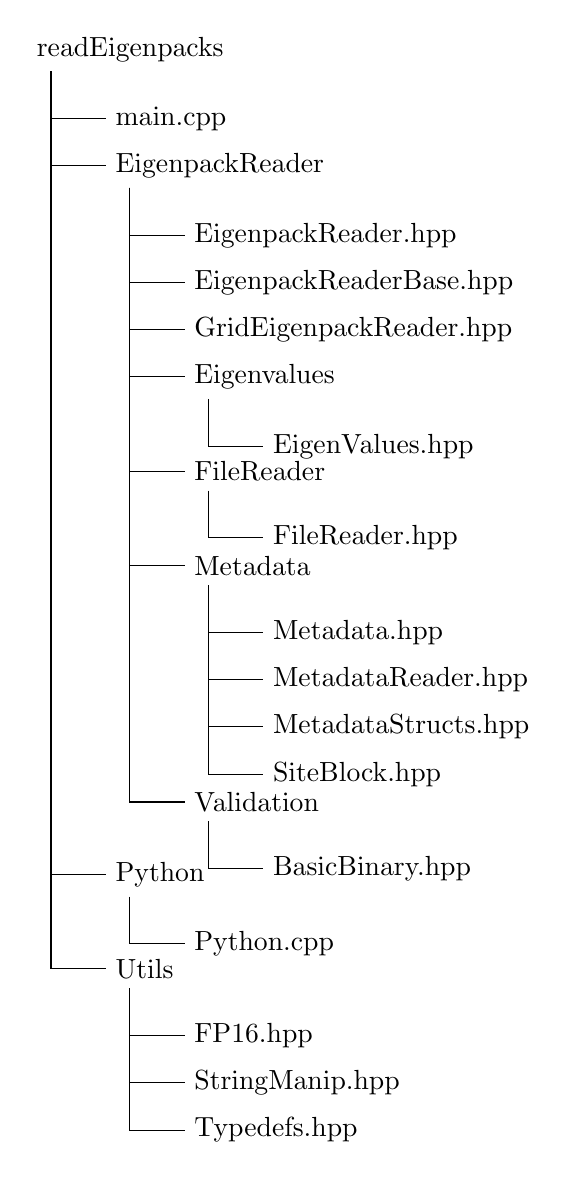
\begin{tikzpicture}[dirtree]
\node {readEigenpacks} 
    child {node {main.cpp}}
    child 
    { 
        node {EigenpackReader}
        child {node {EigenpackReader.hpp}}
        child {node {EigenpackReaderBase.hpp}}
        child {node {GridEigenpackReader.hpp}}
        child 
        { 
            node  {Eigenvalues} 
            child 
            { 
                node {EigenValues.hpp}
            } 
        }
        child 
        { 
            node {FileReader} 
            child 
            {
                node {FileReader.hpp} 
            } 
        }
        child
        {
            node  {Metadata}
            child {node {Metadata.hpp}}
            child {node {MetadataReader.hpp}}
            child {node {MetadataStructs.hpp}}
            child {node {SiteBlock.hpp}}            
        }
        child
        {
            node {Validation}
            child
            {
                node {BasicBinary.hpp}
            }
        }
    }
    child 
    { 
        node {Python}
        child { node {Python.cpp} }
    }
    child 
    { 
        node {Utils}
        child { node {FP16.hpp} }
        child { node {StringManip.hpp} }
        child { node {Typedefs.hpp} }
    };
\end{tikzpicture}
\end{center}
\label{FIGURE::CodeLayout}
\caption{Organisation of the source code.}
\end{figure}

\clearpage
\section{Program Compilation and Running}
\subsection{Compilation}
\begin{itemize}
\item Run autoreconf:\\
\texttt{./bootstrap.sh}.
\item Create an out-of-source build directory:\\
\texttt{mkdir build; cd build}
\item Configure with the following options:\\
\begin{tabular}{p{0.49\textwidth}p{0.49\textwidth}}
\texttt{../configure} &\\
\texttt{--prefix=<path/to/install/program>}&\\
\texttt{--with-grid=<path/to/grid>}&\\
\texttt{--with-hadrons=<path/to/hadrons>}&\\
\texttt{CC=clang}       & \# Whichever compiler was used for Grid \& Hadrons\\
\texttt{CXX=clang++}    & \# Whichever compiler was used for Grid \& Hadrons\\
\texttt{nbasis=250}   & \# Number of basis (fine) vectors. Must exactly equal the number of basis vectors used by the eigenpack.\\
\texttt{concbasis=2}  & \# Number of basis (fine) vectors to convert per batch. Low numbers harm performance, but use less memory.\\
\texttt{conceigen=100}& \# Number of (coarse) eigenvectors to convert per batch. Low numbers harm performance, but use less memory.
\end{tabular}
\item Make and install\\
\texttt{make}\\
\texttt{make install}
\end{itemize}

\subsection{Running}
The program can be ran with the following options:\\
\begin{tabular}{p{0.37\textwidth}p{0.62\textwidth}}
\texttt{path/to/EigenpackConverter} &\\
\texttt{--grid 64.64.64.128} & \# Fine lattice size\\
\texttt{--mpi 1.1.2.2}       & \# MPI layout for the conversion\\
\texttt{--Ls 12}             & \# Lattice Ls extent\\
\texttt{--config 1000}       & \# Configuration number\\
\texttt{--i /path/to/input}  & \# Path to GPT eigenpack (containing metadata.txt)\\
\texttt{--o /path/to/output}  & \# Directory to output Scidac eigenpack to\\
\texttt{--outmode <fmt>} & \# Which format to output data in:
\begin{itemize}
\item none: No output
\item basic: Debug format, do not use
\item hadrons: Scidac format
\end{itemize} 
\end{tabular}

\subsection{Potential Issues}
\subsubsection{Insufficient MPI Ranks}
MPI processes can write a maximum of $2^{32}$ bytes each. Since Scidac eigenvector files typically exceed this, multiple MPI processes are usually needed to successfully write an eigenpack. For example, an eigenpack with eigenvectors that decompress to 18 GiB must be written using at least 9 MPI processes. The program will check the number of MPI processes in use before performing the conversion, and exit if an insufficient number is detected. Typically, enough MPI processes will be usable on a single node to convert an eigenpack.

\subsubsection{Non-factorisable local volumes}
Each file of the GPT eigenpack files corresponds to a contiguous chunk of the lattice. This is given by the `\textbf{s}' parameter in the eigenpack metadata file. The dimensions of this chunk must exactly factorise into the local volume of the grid used to perform the conversion due to current limitations of the conversion implementation. For example, an eigenpack with dimensions of $4\times 3\times 4\times 4$ can only be converted on a grid with a local volume that is a multiple of 4 in the x, z, and t dimensions, and a multiple of 3 in the y dimension. The program will exit with an error message if this condition is not fulfilled.

\end{document}